\section{Security Context}
\label{sec:securitycontext}

In the early days of the internet, everything sent over it was public. If A sent a message to B, anyone on their path through the internet could read it. Email still operates in this model of no privacy. Today, there exist end-to-end encrypted alternatives, most notably the messaging app, Signal. Unfortunately, if their servers are hacked, one of their employees bribed, or an ISP or a government targets you, the attacker can learn when, where and with whom you are talking. Anysphere guarantees metadata privacy, meaning that all information is hidden from everyone — just like an in-person conversation. \cref{fig:metadataprivacy} illustrates the difference.
\xxx[sualeh]{Hmm, this seems like a repeat of the previous paragraph in the introduction.}

\begin{figure}[h!]
    \centering
        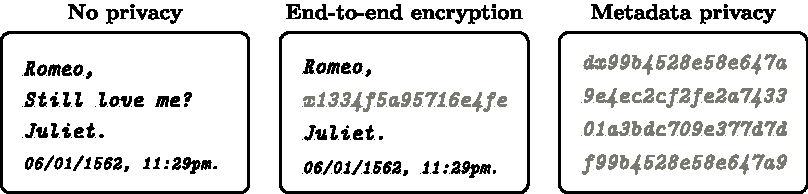
\includegraphics[width=\textwidth]{metadata-privacy.pdf}
\caption{The view of a powerful adversary. With end-to-end encryption, the adversary can still see the metadata.}
\label{fig:metadataprivacy}
\end{figure}

This section describes our desired properties and the threat model we want them to hold in. In short, we guarantee metadata privacy against anyone except the conversation partners themselves.

\subsection{Goals}

The goals below are in reference to an attacker with the capabilities defined in the threat model section (\cref{subsec:threatmodel}).

\textbf{1. Metadata privacy.} An attacker does not learn anything about what messages are being sent when, between whom. This implies that the attacker cannot read messages (because it does not even know that the messages exist). We guarantee one of the strongest possible versions of metadata privacy: formally, an attacker can simulate its view in the real world given only the knowledge of its own messages (see \cref{sec:coreprotocol} for more details).
\xxx[sualeh]{It would be awesome to have a clearer sentence for the formal claim. I have not come up with one yet.}

\textbf{2. Integrity.} An attacker cannot forge a message from anyone, or edit any of the messages being sent.

\textbf{3. Partial resistance to denial-of-service attacks}. An attacker that merely controls a number of users cannot block messages from being delivered. However, we do not guarantee service against an attacker that controls the server or the network.

\textbf{4. Reasonable load on client and server}. The server load is feasible, and users are able to run a client on any commonly sold internet device. It may be allowed for users to adjust their load to their preference.

\subsection{Threat Model}
\label{subsec:threatmodel}


We plan to achieve our goals in the presence of strong adversaries, whose capabilities we define in this section. Our belief in no needless trust means that our threat model is as extensive as possible.

%\begin{table*}[t]
%\centering
%another version below
%\begin{tabular}{||c c c c c c||} 
% \hline
%  Attacker compromises $\cdots$ & Anysphere & Signal & Skiff & Wickr & Onion  \\
% \hline
% Attacker listens on the internet & \checkmark & \checkmark & \checkmark & \checkmark \\ 
% \hline
% Attacker compromises & \checkmark & & & \checkmark & \checkmark \\
% \hline
% Skiff & \checkmark &  &  & & \checkmark\\
% \hline
% Wickr & \checkmark & & & \checkmark & \checkmark\\
% \hline
% Onion & \checkmark & *\footnote{\label{onion}Only guaranteed for non-global adversary} & &\checkmark&\checkmark\\
% \hline
%\end{tabular}
%\caption{Comparing when}
%\end{table*}

% \xxx{add an illustration of a walled garden, with the walls containing only your computer and your friends' computers} 

%Touch on: server, friends, client-side computer, etc.

\textbf{1. The attacker may compromise all servers.} To achieve privacy, we do not put any trust in the server. Our threat model assumes a global adversary who has full control over all servers, and can observe and manipulate all network traffic. This is similar to other anonymous communication schemes based on private information retrieval (for example \cite{ahmad2021addra}, \textsection 2.2), but stronger than most other anonymous communication schemes (e.g. Tor \cite{dingledine2004tor} and Nym \cite{piotrowska2017loopix}, which require partial trust in the servers).

\textbf{2. The attacker may control the entire internet.} See above.

\textbf{3. The attacker may compromise strangers.} We assume that the attacker has control over all clients that are not a contact of a given user, and can send maliciously crafted messages to and from these clients.

\textbf{4. The attacker cannot compromise contacts.} We assume that a user's contacts are trusted, and that the attacker does not have access to their computers. In \cite{angel2018s}, Angel, Lazar and Tzialla describe an attack on a general metadata-private communication system, which shows how to leak metadata in the presence of a compromised contact. The amount of metadata leaked to contacts is small, and we plan to look into measures for handling compromised contacts in the future (see \cref{sec:future}).
% that perfectly hiding metadata while not trusting the user's contacts is computationally prohibitive. <- edited out because we shouldnt have to justify not using this in the threat model.

\textbf{5. The attacker cannot access the user's computer.} We assume that a user's local computer is trusted and is running a correct implementation of our system. In \cref{sec:practical-security} we explain how we can relax this assumption slightly.

\textbf{6. The attacker cannot break standard cryptography.}: Our threat model assumes the security of the standard cryptography primitives we use. This includes Libsodium's AEAD implementation (XSalsa20), and Microsoft SEAL's homomorphic encryption implementation (BFV).

\subsection{Non-goals}
\textbf{1. Not a cryptocurrency.} Anysphere uses advanced cryptography, but not blockchains or cryptocurrencies.

\textbf{2. Not a plugin to an existing ecosystem.} Anysphere is not compatible with existing messaging systems like Signal or Email. This is intentional: interfacing with legacy systems would mean accepting their (much lower) standards of security and privacy.

\textbf{3. Not steganographic.} Anysphere does not make an attempt to hide who is using our service.

